\chapter{Concept Activation Vector Method} \label{chap:cav}

\section{Introduction}
The Concept Activation Vector (CAV) method is a technique to learn meaningful directions from the hidden layers of a neural network \cite{cav_def}.Test with Concept Activation Vectors (TCAV) \nomenclature[Z]{TCAV}{Test with Concept Activation Vectors} was proposed to measure how sensitive a neural network is to a human-defined concept \cite{tcav}. For example, given a classifier that predicts whether an image contains zebra, a CAV with the concept `stripes' could be used to measure how important stripes are to the classifier's decision.

Xizi worked on using CAV to measure bias within a feature-based DDN grading system \cite{feature_bias}, which is built on the fact that the CAV method could measure bias. The research in \cite{tcav} has identified positive linkage of the concept `female' with the classification of `aprons', which shows a gender bias over objects. Hence, it is proposed that CAV could also measure whether these human concepts would affect the grading process of the models.

The rest of this chapter would discuss the concept of CAV - how it is extracted from the models, and how it is used to measure bias.

\section{Extraction of CAV}
When training the models in chapter \ref{chap:graders}, a supervised training data ($\mathcal{D}$) with intermediate vector $\mathbf{\hat{x}}^{(i)}$ and the true score $y^{(i)}$. The neural network ($\mathcal{F}$) is trained with $\mathbf{\hat{x}}^{(i)}$ and the network parameters $\boldsymbol{\theta}$. For DNN, $\mathcal{F}$ outputs the predicted score $\hat{y}^{(i)}$ in equation \ref{eq:DNN}. For DDN, $\mathcal{F}$ outputs the predicted Gaussian distribution with mean $\mu^{(i)}$ and standard deviation $\sigma^{(i)}$ in equation \ref{eq:DDN}.

\begin{equation} \label{eq:DNN}
    \mathcal{D} = \left\{\{\mathbf{\hat{x}}^{(i)},y^{(i)}\}\right\}_{i=1}^{N}; \qquad \mathbf{\hat{y}}^{(i)} = \mathcal{F}_{\text{DNN}}(\mathbf{x}^{(i)}, \boldsymbol{\theta})
\end{equation}

\begin{equation} \label{eq:DDN}
    \mathcal{D} = \left\{\{\mathbf{\hat{x}}^{(i)},y^{(i)}\}\right\}_{i=1}^{N}; \qquad \mu^{(i)}, \sigma^{2(i)} = \mathcal{F}_{\text{DDN}}(\mathbf{\hat{x}}^{(i)}, \boldsymbol{\theta})
\end{equation}

$\mathcal{F}$ could be split into two parts: the transformation from the input to a hidden layer output after the activation function ($\mathbf{h}^{(i)}$), and from $\mathbf{h}^{(i)}$ to the output. Equation \ref{eq:DNN_split} and \ref{eq:DDN_split} shows the split for DNN and DDN respectively.

\begin{equation} \label{eq:DNN_split}
    \mathbf{h}^{(i)} = \mathcal{F}_{\text{h,DNN}}(\mathbf{\hat{x}}^{(i)}, \boldsymbol{\theta}); \qquad \mathbf{\hat{y}}^{(i)} = \mathcal{F}_{\text{y,DNN}}(\mathbf{h}^{(i)}, \boldsymbol{\theta})
\end{equation}

\begin{equation} \label{eq:DDN_split}
    \mathbf{h}^{(i)} = \mathcal{F}_{\text{h,DDN}}(\mathbf{\hat{x}}^{(i)}, \boldsymbol{\theta}); \qquad \mu^{(i)}, \sigma^{(i)} = \mathcal{F}_{\text{y,DDN}}(\mathbf{h}^{(i)}, \boldsymbol{\theta})
\end{equation}

$\left\{ \mathbf{h}^{(i)} \right\}_{i=1}^N$ can be split into positive and negative examples. For example, say `Thai' as the L1 language is a concept. $\boldsymbol{h_{pos}^{(i)}}$ originates from Thai candidates, and $\boldsymbol{h_{neg}^{(i)}}$ originates from non Thai candidates.

A simple linear classifier is trained among $\boldsymbol{h}$, with a linear decision boundary separating positive and negative outputs. The classifier is trained with hinge-loss minimization with L2-norm penalty, which penalizes extreme weights. The loss function is in equation \ref{eq:hinge-loss}:

\begin{equation} \label{eq:hinge-loss}
    \mathcal{L}(\boldsymbol{d^{(c)}}, b) = \sum_{i=1}^{N} w_{t^(i)} \mathrm{max} \{0, 1 - t^{(i)}(\boldsymbol{d}^{(c)T}\boldsymbol{h}^{(i)} + b)\} + \alpha \|\boldsymbol{d^{(c)}}\|_2^2
\end{equation}

where $t^{(i)} \in \{1, -1\}$ is the target label, where $t = 1$ for positive examples and $t = -1$ for negative examples, $w_{t^{(i)}}$ is the weighting for the i-th sample with target label $t^{(i)}$, and $\alpha$ is the regularization parameter that controls the strength of the L2-norm penalty.

The loss function maximizes the margin, as it encourages pushing as many data points away from the margin as possible. The L2-norm penalty is used to prevent overfitting from maximizing a particular weight, through adding a regularization term to the loss function. The linear decision boundary could be defined with the equation $\boldsymbol{d}^{(c)T}\boldsymbol{h} + b = 0$. The concept activation vector $\boldsymbol{d^{(c)}}$ of concept $c$ is the normal vector to the decision boundary. A 2-dimensional example is illustrated in figure \ref{fig:linear}.

\begin{figure}[H]
    \centering
    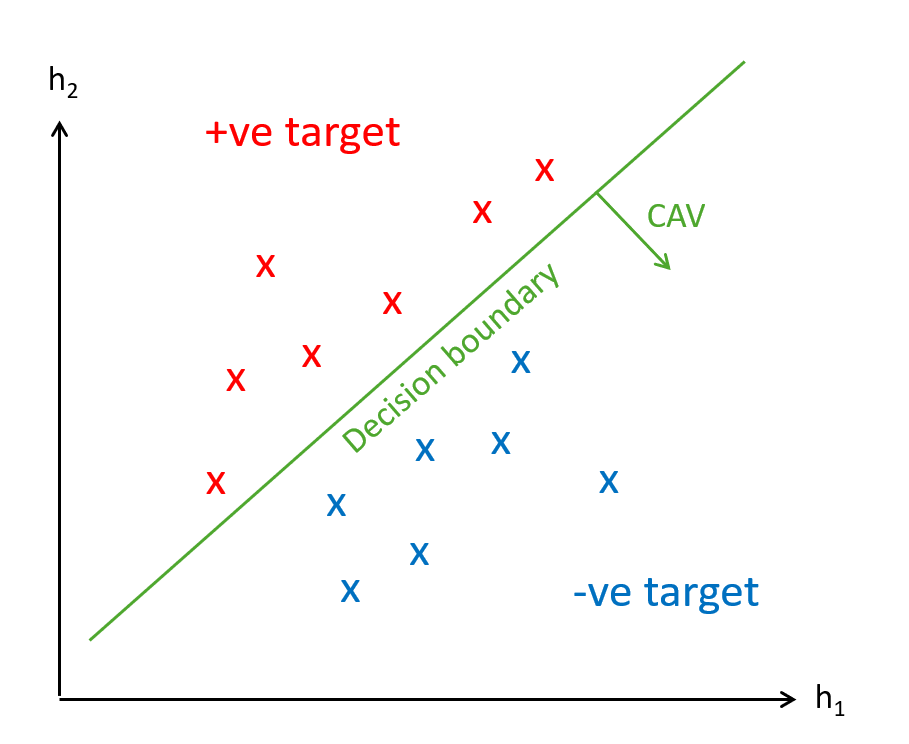
\includegraphics[width=0.4\textwidth]{linear.png}
    \caption{Illustration of CAV extraction. $h_1$ and $h_2$ represents  $\boldsymbol{h}$'s two dimensions}
    \label{fig:linear}
\end{figure}

The value of $w_{t^{(i)}}$ depends on the type of weighting used. In previous work, no weighting is used when extracting CAV, which essentially set $w_{t^{(i)}} = 1$ \cite{feature_bias}. Balanced weighting, on the other hand, set $w_{t^{(i)}} \propto \frac{1}{N_{i}}$, with $N_i$ being the number of samples with the same target label as $t^{(i)}$. Since balanced weighting assigns higher weights to underrepresented classes, it ensures that the classifier does not become biased towards the majority class. Since the use of weighting is found to generally improves the performance of machine learning methods \cite{balanced}, this paper would extract CAV with both methods, and compare the results.

\section{Perturbation of CAV}

Perturbation of the network is done by adding $\boldsymbol{\Delta h}$, which is along the CAV, to the activation layer's vector $\boldsymbol{h}$. The calculation of $\boldsymbol{\Delta h}$ is represented in equation \ref{eq:perturb}.

\begin{equation} \label{eq:perturb}
    \boldsymbol{\Delta h}^{(c)} = \left(\frac{1}{N}\sum_{i=1}^{N} \|\boldsymbol{h}^{(i)}\|_{2}) \right) \frac{ \boldsymbol{d}^{(c)}}{\| \boldsymbol{d}^{(c)}\|_2}
\end{equation}

Perturbation along the CAV could be represented as a linear combination of the CAV and the original vector $\boldsymbol{h}$. Figure \ref{fig:perturbation} illustrates the perturbation of a 2-dimensional activation vector, and the perturbation could be added to the system in the form of equation \ref{eq:add_perturbation}.
\begin{figure}[H]
    \centering
    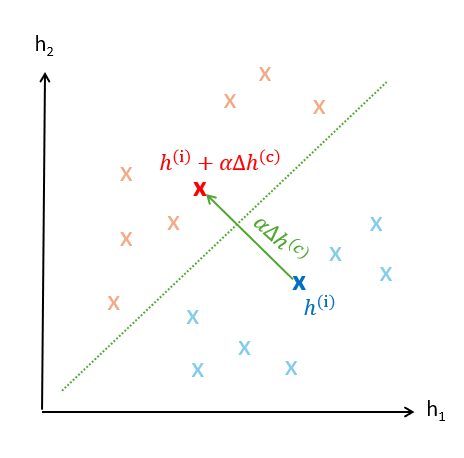
\includegraphics[width=0.35\textwidth]{perturbation.png}
    \caption{Illustration of CAV perturbation}
    \label{fig:perturbation}
\end{figure}

\begin{equation} \label{eq:add_perturbation}
    \mathcal{F}_{y}(\boldsymbol{h}^{(i)}; \boldsymbol{\theta}) \qquad \rightarrow \qquad \mathcal{F}_{y}(\boldsymbol{h}^{(i)} + \alpha \boldsymbol{\Delta h}^{(c)}; \boldsymbol{\theta})
\end{equation}

where $\alpha$ is the perturbation factor, a hyperparameter that controls the strength of the perturbation.

As illustrated in figure \ref{fig:perturbation}, $\boldsymbol{\Delta h}^{(c)}$ moves the activation vector closer to the positive examples, which makes $\boldsymbol{h}$ more `positive' in the sense of the concept. For concepts that are not related to the grading process, the perturbation would not change the prediction of an unbiased model. However, for concepts that are related to the grading process, the perturbation should change the prediction. For example, perturbing the CAV of `male' makes a sample more `male' in the sense of the concept. As gender is not an assessing criteria, the predicted score should not change. In contrast, perturbing the CAV of `high speaking grade' makes the sample possess qualities of a stronger candidate, which should improve the prediction.

\section{Gradient-based Method} \label{sec:gradient}

As illustrated in figure \ref{fig:relevant}, when $\boldsymbol{\Delta h}^{(c)}$ changes the score prediction, the direction is said to be align with $\frac{\partial \mathcal{F}_y}{\partial \boldsymbol{h}}$, the gradient of the network with respect to the activation vector of a particular layer. \nomenclature[A]{$\frac{\partial \mathcal{F}_y}{\partial \boldsymbol{h}}$}{Gradient of the Network With Respect to the Activation Vector of a Particular Layer} Otherwise, as shown in figure \ref{fig:irrelevant}, the direction is said to be orthogonal to $\frac{\partial \mathcal{F}_y}{\partial \boldsymbol{h}}$. The more aligned $\boldsymbol{\Delta h}^{(c)}$ is with the gradient, the greater the change in the predicted score after perturbation. For DNN, $\frac{\partial \mathcal{F}_y}{\partial \boldsymbol{h}} = \frac{\partial \mathbf{\hat{y}}}{\partial \boldsymbol{h}}$. For DDN, as the focus is on the predicted score and not the variance, $\frac{\partial \mathcal{F}_y}{\partial \boldsymbol{h}} = \frac{\partial \mathbf{\mu}}{\partial \boldsymbol{h}}$. As $\boldsymbol{\Delta h}^{(c)}$ is a scalar multiple of the CAV $\boldsymbol{d}^{(c)}$, the alignment could simply be compared between $\boldsymbol{d}^{(c)}$ and $\frac{\partial \mathcal{F}_y}{\partial \boldsymbol{h}}$.

\begin{figure}[H]
    \centering
    \begin{subfigure}{0.45\textwidth}
        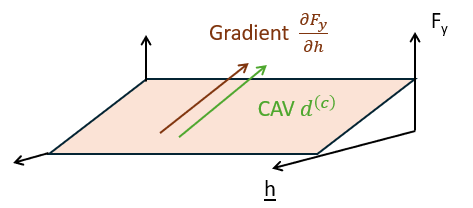
\includegraphics[width=\textwidth]{relevant.png}
        \caption{Gradient direction with CAV of relevant concept}
        \label{fig:relevant}
    \end{subfigure}
    \hfill
    \begin{subfigure}{0.45\textwidth}
        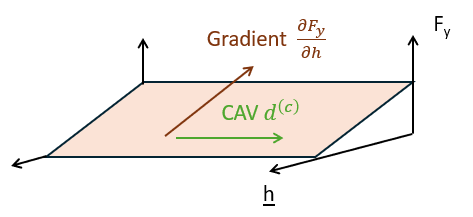
\includegraphics[width=\textwidth]{irrelevant.png}
        \caption{Gradient direction with CAV of irrelevant concept}
        \label{fig:irrelevant}
    \end{subfigure}
\end{figure}

Cosine distance ($\cos(\boldsymbol{a}, \boldsymbol{b})$) is used to compute the alignment. The cosine distance is defined in equation \ref{eq:cosine_distance}:

\begin{equation} \label{eq:cosine_distance}
    \cos(\boldsymbol{a}, \boldsymbol{b}) = 1 - \frac{\boldsymbol{a}^T \boldsymbol{b}}{\|\boldsymbol{a}\|_2 \|\boldsymbol{b}\|_2}
\end{equation}

which is 1 when $\boldsymbol{a}$ and $\boldsymbol{b}$ are orthogonal, and deviates from 1 when they are aligned. For an unbiased system's measurement with CAV of irrelevant concepts, the cosine distance should be 1.

The cosine distance between $\boldsymbol{d}^{(c)}$ and $\frac{\partial \mathcal{F}_y}{\partial \boldsymbol{h}}$ could be measured in two ways. The first way is between the CAV $\boldsymbol{d}^{(c)}$ and the average gradients $\frac{\partial \mathcal{F}_y}{\partial \boldsymbol{h}}$ from all data in equation \ref{eq:grad_del}, which is a faster method to compute for the gradient distance. Another way, the average gradient cosine distance method \nomenclature[A]{$\mathcal{B}^{(c)}_{gr}$}{Average Gradient Cosine Distance}, is averaging the cosine distance of each CAV $\boldsymbol{d}^{(c)}$ and gradient $\frac{\partial \mathcal{F}_y}{\partial \boldsymbol{h}}$ pair, as shown in equation \ref{eq:grad_gr}. This method allows isolation of gradient distance for each sample, providing more insights for analysis.

\begin{equation} \label{eq:grad_del}
    \mathcal{B}^{(c)}_{\nabla} = \cos\left(\boldsymbol{d}^{(c)}, \frac{1}{N} \sum_{i=1}^{N} \frac{\partial \mathcal{F}_y(\boldsymbol{h})}{\partial \boldsymbol{h}}\vert_{\boldsymbol{h^{(i)}}} \right)
\end{equation}

\begin{equation} \label{eq:grad_gr}
    \mathcal{B}^{(c)}_{gr} = \frac{1}{N} \sum_{i=1}^{N} \mathcal{B}^{(ci)}_{gr} = \frac{1}{N} \sum_{i=1}^{N}\cos\left(\boldsymbol{d}^{(c)}, \frac{\partial \mathcal{F}_y(\boldsymbol{h})}{\partial \boldsymbol{h}}\vert_{\boldsymbol{h^{(i)}}} \right)
\end{equation}

\section{Assumptions}
To allow the CAV method to accurately measure the bias, the components in the workflow (input data, model under investigation, linear classifier for CAV extraction) should satisfy the following assumptions:

The true score from human graders should be unbiased. CAV only has the ability to detect presence within a trained model, but it cannot isolate whether the cause is due to the data or the model itself. If the input data is biased, even if the model is not inherently biased, the trained model would still become biased. A way to verify the assumption is to check the average score of input data of different concepts (see Section \ref{sec:data_construction}). For concepts irrelevant to performance, the average score should be similar.

The model should be reasonably accurate. If the model is inaccurate, the activation $\boldsymbol{h}$ would unlikely be representing the concepts accurately. To verify the assumption, the model's accuracy could be checked with the testing set. The model should be able to predict the score with low error.

The activations should be linearly separable. There could be a case in figure \ref{fig:overlap} where the activations $\boldsymbol{h}$ are simply too overlapped, such that any classifier could not differentiate between the two classes. Even if the activations $\boldsymbol{h}$ are separable, it should be by a linear classifier, rather than a non-linear decision boundary in figure \ref{fig:non_linear}, as the CAV is the orthogonal vector to the decision boundary. Otherwise, a linear decision boundary with low accuracy would be trained, shown as the dotted line in the figure. The more accurate the linear classifier, the more representative the CAV is for the related concept. This could be verified by checking the accuracy of the linear classifier in differentiating positive and negative examples.

\begin{figure}[H]
    \centering
    \begin{subfigure}{0.45\textwidth}
        \centering
        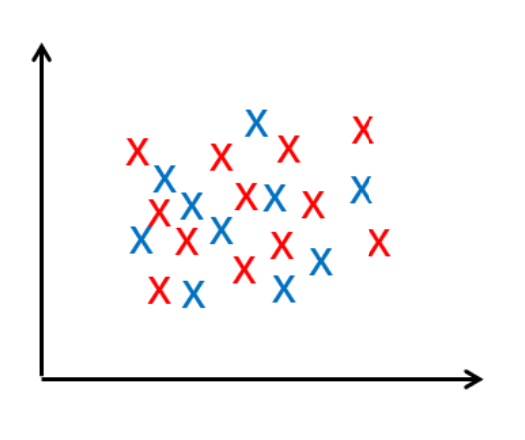
\includegraphics[width=0.6\textwidth]{overlap.png}
        \caption{Activations that are closely overlapped}
        \label{fig:overlap}
    \end{subfigure}
    \hfill
    \begin{subfigure}{0.45\textwidth}
        \centering
        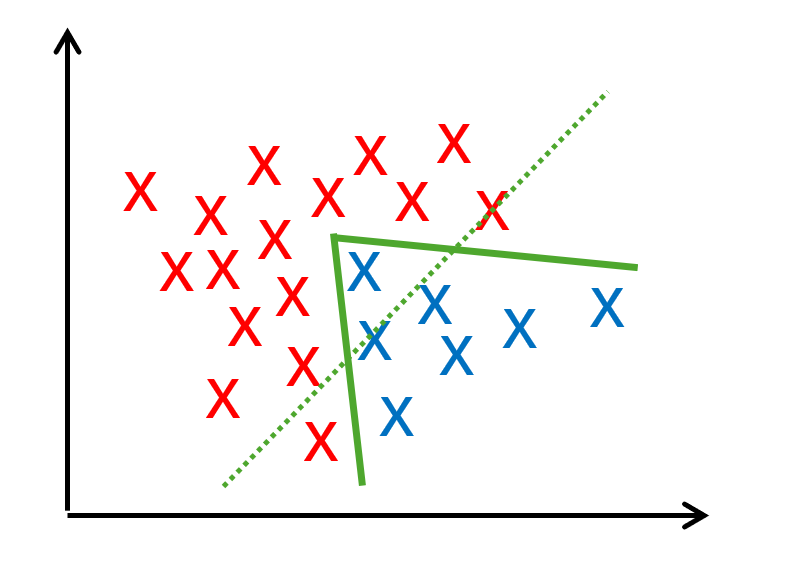
\includegraphics[width=0.6\textwidth]{non_linear.png}
        \caption{Activations with non-linear decision boundary}
        \label{fig:non_linear}
    \end{subfigure}
\end{figure}

\section{Summary}
This chapter discussed the CAV method, highlighting how it could be used to detect bias in a model. The mathematical details on how to extract CAV from the model, how to perturb the activation along the CAV, and how to measure bias through alignment of CAV with the gradient were discussed. The assumptions of the CAV method were also discussed, including that the input data is unbiased and that the activation is linearly separable. This outlines the foundation to measure the models' bias in the upcoming chapters.